\documentclass{article}

% set font encoding for PDFLaTeX or XeLaTeX
\usepackage{ifxetex}
\ifxetex
  \usepackage{fontspec}
\else
  \usepackage[T1]{fontenc}
  \usepackage[utf8]{inputenc}
  \usepackage{lmodern}
    \usepackage{graphicx}
  \usepackage{float}
\fi

% used in maketitle
\title{Evaluación 2}
\author{Eduardo Hernández\\Universidad de Sonora\\Lic. en Física}

% Enable SageTeX to run SageMath code right inside this LaTeX file.
% documentation: http://mirrors.ctan.org/macros/latex/contrib/sagetex/sagetexpackage.pdf
% \usepackage{sagetex}

\begin{document}
\maketitle
\section{actividad1}
en esta actividad se nos proporcionó un código que calculaba el valor de la exponencial, así como su aproximación mediante la serie de Maclaurin.

El programa solo daba los primeros 20 términos necesarios para calcular el valor de e a la primera potencia.

el código muestra es como sigue
\begin{verbatim}
! ----------- Begin ------------
!taylor.f90
program taylor

    implicit none                  
real (kind=8) :: x, exp_true, y
    real (kind=8), external :: exptaylor
    integer :: n

    n = 20               ! number of terms to use
    x = 1.0
    exp_true = exp(x)
    y = exptaylor(x,n)   ! uses function below
    print *, "x = ",x
    print *, "exp_true  = ",exp_true
    print *, "exptaylor = ",y
    print *, "error     = ",y - exp_true

end program taylor

!==========================
function exptaylor(x,n)
!==========================
    implicit none

    ! function arguments:
    real (kind=8), intent(in) :: x
    integer, intent(in) :: n
    real (kind=8) :: exptaylor

    ! local variables:
    real (kind=8) :: term, partial_sum
    integer :: j

    term = 1.
    partial_sum = term

    do j=1,n
        ! j'th term is  x**j / j!  which is the previous term times x/j:
        term = term*x/j   
        ! add this term to the partial sum:
        partial_sum = partial_sum + term   
        enddo
     exptaylor = partial_sum  ! this is the value returned
end function exptaylor
! --------  End -------------
\end{verbatim}

los datos que arrojaba este programa son como sigue
\begin{verbatim}
 x =    1.0000000000000000     
 exp_true  =    2.7182818284590451     
 exptaylor =    2.7182818284590455     
 error     =    4.4408920985006262E-016
\end{verbatim}
\section{actividad2}
La actividad dos nos pedía realizar la aproximación del exponencial con npts=100 y en un x0=0 y X=10 el código me quedó de la siguiente manera..
\subsection{código}
\begin{verbatim}

subroutine Ap(x_1,n,y)
  implicit none
  integer(kind=8) ,intent (in)::n !número de términos
  real (kind=8),intent (in) ::x_1
  real (kind=8), intent (out)::y
  real (kind=8),dimension(100)::r,x !acumulador
  !variables locales
  real(kind=8)::term, partial_sum
  integer::i
  !termino inicial y la suma de las terminos
  term=1.0
  do i=1,100
     x(i)=float(i)/10.0
     write(1,*) x(i), term
  end do
  write(1,*) ''
  r=0
 partial_sum=term
 !ciclo el número de términos
 do i=1,n
    !calcular el factorial
    term=term*x_1/float(i)
    !agrega este término a la suma parcial
    partial_sum=partial_sum + term
    r(i)=partial_sum
    y=r(i)
    end do
  end subroutine Ap
!iniciamos programa  
program Taylor
  implicit none
  real (kind=8)::y
  integer(kind=8) ::i,j,n
  real(kind=8), dimension(100):: x,exp_true
  
  open(1,file='taylor.dat',status='unknown')
  
  exp_true=exp(x)
  do n=1,15,2
     do j=1,100
        x(j)=float(j)
        x(j)=x(j)/10.0
    !llamamos a la subrutina
      call Ap(x(j),n,y)
        write(1,2) x(j) ,y
          2 format(1x,F12.8,F12.8) 
        write(1,*)''
         end do
end do
 close(1)
end program Taylor
  
\end{verbatim}
Y al graficarlo quedó como sigue:
\begin{figure}[h!]
  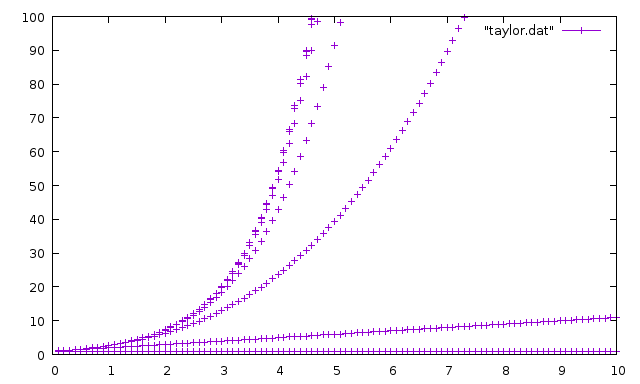
\includegraphics[width=\linewidth]{exp.png}
  \caption{final}
  \label{fig:boat1}
  \end{figure}
\section{actividad3}
aún no termino la actividad 3, pero el código que llevo es como sigue (está incompleto):
\begin{verbatim}

subroutine Ts(x_1,n,y)
    implicit none
    integer(kind=8), intent(in) ::n !número de términos
    real (kind=8), intent(in):: x_1
    real(kind=8), intent(out)::y
    real(kind=8), dimension(100)::r,x !acumulador
    !variables locales
    real(kind=8)::term,partial_sum
    integer::i
    !término inicial y suma de términos
    term=1.0
    r=0
    partial_sum=term
    !bucle para el número de términos
    do i=1,n
       !calcular el factorial
       term=((-1)**(i)*((i)+1))/((float(i)*2)+1)
       !agregar el término a la suma parcial
       partial_sum=partial_sum-term
       r(i)=partial_sum
       y=r(i)
    end do
  end subroutine Ts
  !iniciamos programa
  program TaylorS
    implicit none
    real(kind=8),parameter:: pi=3.1415
    real(kind=8)::y
    integer(kind=8) i,j,n
    real(kind=8), dimension(100)::x, true_sin
    open(3,file='AproxSin.dat',status='unknown')
true_sin=sin(pi*x/180)
do n=1,30,2
   do j=1,100
      x(j)=float(j)
      x(j)=x(j)/10.0
      !llamamos a la subrutina
      call TS(x(j),n,y)
      write(3,2) x(j) , y
2     format(2x,F12.8,F12.8)
      write(3,*) ''
   end do
end do
close(3)
end program TaylorS


\end{verbatim}
\end{document}
